\documentclass[
    10pt,
    aspectratio=169,
    xcolor={dvipsnames},
    spanish,
    % handout,
    % notes=only,
    % notes,
    ]{beamer}

% BEAMER SETTINGS
\setbeamerfont{section in toc}{size=\normalsize, shape=\bfseries}
\mode<presentation>{
    \usetheme{Antibes}
    \setbeamercovered{transparent}
    \usecolortheme{rose}
    \setbeamertemplate{navigation symbols}{}
    }

% PACKAGES
% \usepackage[spanish]{babel}  % uncomment for Spanish support
\usepackage{tikz,pgfplots}
\pgfplotsset{compat=1.13}
\usetikzlibrary{calc}
\usepackage{subcaption}
\usepackage{graphicx}
\graphicspath{{figures}}
\usepackage{booktabs}
\usepackage{upgreek}
\usepackage{commath}
\usepackage{amsmath,amsthm,amssymb,mathtools,mathrsfs}
\usepackage{cancel}
\usepackage{fontawesome5}
\usepackage{enumerate}
\usepackage{tensor}
\usepackage[font=footnotesize]{caption}
\usepackage{wasysym}

\usepackage[skins,theorems]{tcolorbox}
\tcbset{
    highlight math style={
        enhanced,
        coltext=black,
        colframe=black,
        colback=lightgray,
        arc=0pt,
        boxrule=.5pt
        }
}

% REFERENCES AND OTHERS
\usepackage{aas_macros}
\usepackage{natbib}
\bibpunct{(}{)}{;}{a}{}{,}

\usepackage{siunitx}
\sisetup{
    range-phrase=\text{--},
    range-units=single,
    separate-uncertainty=true,
    print-unity-mantissa=false
    }
\DeclareSIUnit{\gauss}{G}
\DeclareSIUnit{\jansky}{Jy}
\renewcommand{\figurename}{Fig.}

\usepackage{hyperref}
\hypersetup{
    % bookmarks=true,
    unicode=true,
    pdftoolbar=true,
    pdfmenubar=true,
    pdffitwindow=false,
    pdfstartview={FitH},
    pdftitle={ISI-Free Linear Combination Pulses with Better Performanc},
    pdfauthor={Erik Saez A.},
    pdfcreator={Erik Saez A.},
    pdfnewwindow=true,
    colorlinks=true,
    linkcolor=RoyalBlue,
    citecolor=RoyalBlue,
    urlcolor=RoyalBlue
    }

\title[Auxiliar \#2 - Oscilaciones Armónicas]{\bfseries Auxiliar \#2 - Oscilaciones Armónicas}
\subtitle{Introducción a la Física Moderna (F1100-5)}
\author[Erik Saez A.]{Erik Saez A. - Javiera Toro}
\institute[UChile]{Departamento de Ingeniería Eléctrica \\ Universidad de Chile}

\date{\today}

\begin{document}

\begin{frame}
  \titlepage
  \centering
  \faIcon{envelope} \href{mailto:erik.saez@ug.uchile.cl}{erik.saez@ug.uchile.cl} \hspace{.2cm}
\end{frame}

\begin{frame}{Contenidos}
  \tableofcontents
\end{frame}

\section{Resumen}

\begin{frame}{Definiciones Básicas}
  \begin{block}{Ondas sinusoidales}
    \footnotesize
    Las ondas sinusoidales son un tipo de onda que se caracteriza por tener una forma de onda suave y periódica, descrita matemáticamente por funciones seno o coseno y son por lo general soluciones de los movimientos armónicos simples (M.A.S).
  \end{block}
  
    \begin{columns}[T,totalwidth=\textwidth]
      \begin{column}{0.5\textwidth}
        \scriptsize
        \begin{block}{Elementos que caracterizan una onda}
          \vspace{-0.3em}
          \begin{center}{\normalsize{\( y(t)=A\cos(\omega t + \phi) \)}}\end{center}
          \vspace{-0.6em}
          % Distribuimos los elementos en dos columnas para mejorar el equilibrio visual
          \begin{columns}[T,onlytextwidth]
            \begin{column}{0.4\textwidth}
              \setlength{\itemsep}{2pt}\setlength{\parskip}{0pt}
              \begin{itemize}
                \item \textbf{A}: Amplitud (máximo)
                \item \textbf{T}: Período [s]
                \item \textbf{f}: Frecuencia [Hz] (ciclos/s)
              \end{itemize}
            \end{column}
            \begin{column}{0.5\textwidth}
              \setlength{\itemsep}{2pt}\setlength{\parskip}{0pt}
              \begin{itemize}
                \item \textbf{$\omega$}: Frec. angular [rad/s]
                \item \textbf{$\lambda$}: Longitud de onda
                \item \textbf{$\phi$}: Fase inicial
              \end{itemize}
            \end{column}
          \end{columns}
          \vspace{-0.6em}
          \begin{center}\( f = \tfrac{1}{T} = \tfrac{\omega}{2\pi} \)\end{center}
        \end{block}
      \end{column}
      \begin{column}{0.42\textwidth}
        \centering
        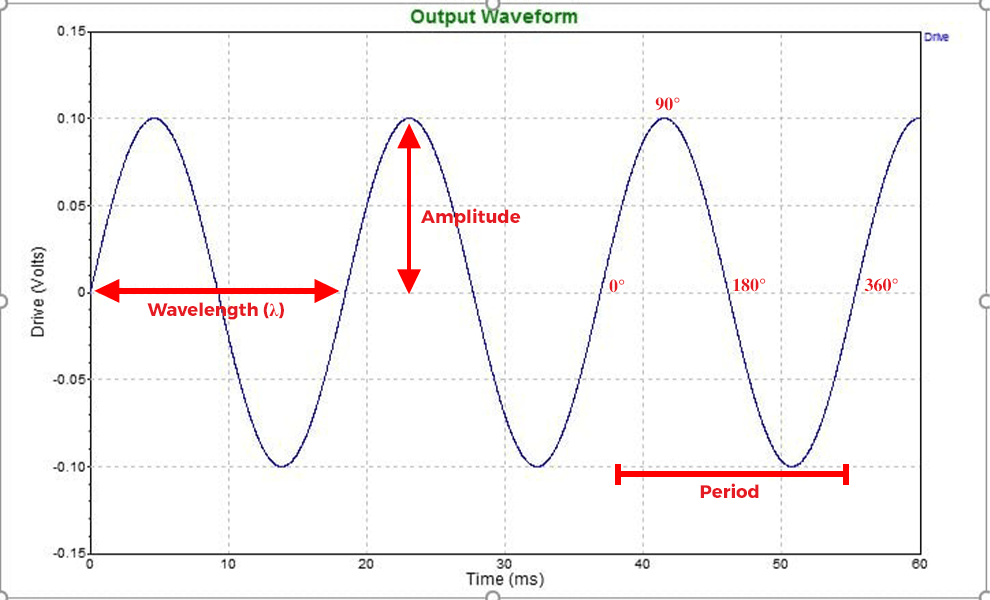
\includegraphics[width=\textwidth]{Auxiliar_1_5.png}
      \end{column}
    \end{columns}
\end{frame}

% =====================================
\begin{frame}{M.A.S.: Ecuación y Solución}
  \footnotesize
  \begin{columns}[T]
    \begin{column}{0.58\textwidth}
      \begin{block}{EDO del M.A.S.}
        Una \textbf{ecuación diferencial ordinaria (EDO)} relaciona una función   desconocida y sus derivadas respecto de una sola variable independiente. La forma más común que encontraremos es la EDO lineal homogénea de 2° orden:
        \begin{equation*}
          m\ddot x + kx = 0 \;\Longleftrightarrow\; \ddot x + \frac{k}{m}x = 0
        \end{equation*}
        \noindent Frecuencia angular $\omega^2=\tfrac{k}{m} \;\Rightarrow\; \omega=\sqrt{\tfrac{k}{m}}$, que cuantifica la rapidez de la oscilación.\vspace{-2pt}
      \end{block}
      \begin{block}{Posición de equilibrio}
        La \textbf{posición de equilibrio} $x_{\text{eq}}$ es aquella en la que la fuerza neta (y por ende la aceleración) se anula: $m\ddot x=0$, lo que implica que:\begin{align}
          \ddot{x}= \dot{x} = 0
        \end{align}
      \end{block}
    \end{column}
    \begin{column}{0.45\textwidth}
      \begin{block}{Derivadas útiles}
        Cambio de variable respecto al equilibrio:\\[-2pt]
        \[
          \begin{aligned}
            y(t) &= x(t)-x_{\text{eq}},\\
            \dot y(t) &= \dot x(t),\\
            \ddot y(t) &= \ddot x(t).
          \end{aligned}
        \]
      \end{block}
      \begin{block}{Solución general y derivada (conocida)}
        Para $\ddot x + \omega^2 x=0$:
        \[
          \begin{aligned}
            x(t) &= A\cos(\omega t)+B\sin(\omega t),\\
            \dot x(t) &= -A\omega\sin(\omega t)+B\omega\cos(\omega t).
          \end{aligned}
        \]
        C.I.: $x(t= 0)=x_0 \Rightarrow A=x_0$, $\;\dot x(0)=v_0 \Rightarrow B=v_0/\omega$.
      \end{block}
    \end{column}
  \end{columns}
\end{frame}
% ===================================

% =====================================
\section{Pregunta 1}

% ------------------ Ejercicio 1 ------------------
\begin{frame}{Ejercicio 1: Corcho flotante}
  \begin{columns}[T,totalwidth=\textwidth]
    \begin{column}{0.60\textwidth}
      \begin{block}{Enunciado pregunta 1}
        Corcho cilíndrico de radio $R$ y altura $H$ se deja en una piscina en reposo hasta alcanzar su posición de equilibrio.
        \begin{itemize}
          \item Calcular la posición de equilibrio.
          \item Si se perturba ligeramente y en $t=0$ está en $x_0$ con velocidad $v_0$, hallar $x(t)$.
        \end{itemize}
        Datos: gravedad $g$ y fuerza de empuje $F_e=\rho g V$, con $\rho$ densidad del agua y $V$ volumen sumergido.
      \end{block}
    \end{column}
    \begin{column}{0.40\textwidth}
      \centering
       \vspace*{1cm}
      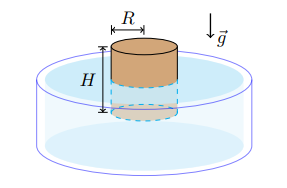
\includegraphics[width=0.9\textwidth]{Auxiliar_1_1 copy.png}
    \end{column}
  \end{columns}
\end{frame}
\section{Pregunta 2}
% ------------------ Ejercicio 2 ------------------
\begin{frame}{Ejercicio 2: Masa entre dos resortes}
  \begin{block}{Enunciado pregunta 2}
    Bloque de masa $M$ entre dos resortes ideales de constantes $k$ y $2k$ (longitudes naturales nulas), sin fricción, movimiento 1D. Inicialmente en equilibrio con velocidad $V$ hacia la derecha.
    \begin{itemize}
      \item Frecuencia angular $\omega$ y amplitud.
      \item Expresión de $x(t)$.
      \item Al cortarse el resorte derecho en su máxima elongación, tiempo hasta el choque con la pared izquierda.
    \end{itemize}
  \end{block}
  \vspace{2pt}
  \centering
  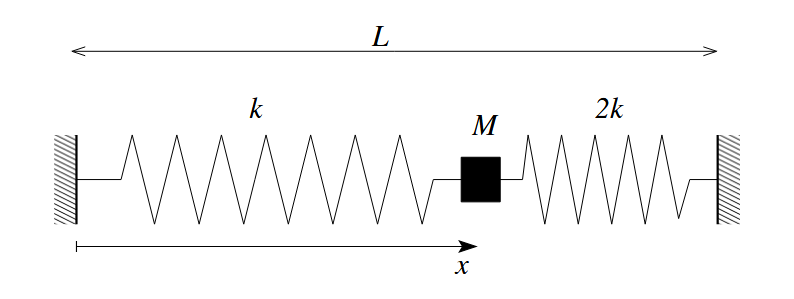
\includegraphics[width=0.6\textwidth]{Auxiliar_1_2 copy.png}
\end{frame}
\section{Pregunta 3}
% ------------------ Ejercicio 3 ------------------
\begin{frame}{Ejercicio 3: Cavidad óptica}
  \footnotesize
  \begin{columns}[T,totalwidth=\textwidth]
    \begin{column}{0.55\textwidth}
      \begin{block}{Enunciado Pregunta 3}
        Una cavidad óptica, elemento básico para construir un láser, puede hacerse usando un espejo plano (Espejo 1) y uno esférico cóncavo (Espejo 2), como en la figura.
        \begin{enumerate}
          \item Con $s_1=5\,\mathrm{m}$, $s_2=20\,\mathrm{m}$, $R=10\,\mathrm{m}$ y altura del peón $h_1=5\,\mathrm{cm}$, determine las imágenes del peón por ambos espejos: si son reales/virtuales, invertidas/derechas y su tamaño.
          \item Use estas dos imágenes como nuevos objetos para generar dos nuevas imágenes; repita el razonamiento para explicar por qué aparecen infinitas imágenes al enfrentar dos espejos.
        \end{enumerate}
      \end{block}
    \end{column}
    \begin{column}{0.40\textwidth}
      \centering
  % bajar solo la imagen de la Pregunta 3
  \vspace*{1cm}
      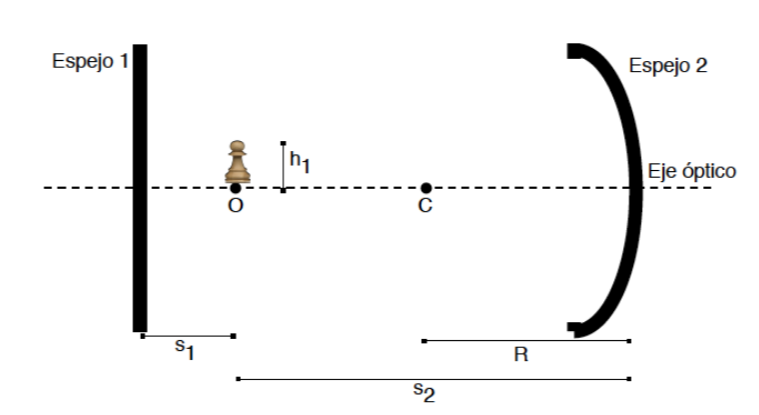
\includegraphics[width=1\textwidth]{Auxiliar_1_5 copy.png}
    \end{column}
  \end{columns}
\end{frame}

\end{document}
